\documentclass[14pt, a4paper]{extarticle}
\usepackage{GOST}
\usepackage{array}
\usepackage{verbatim}
\usepackage[detect-all]{siunitx}
\usepackage{amsmath}
\usepackage{amssymb}
\usepackage[utf8]{inputenc}
\usepackage{hyperref}
\usepackage{tempora}

\makeatletter
\renewcommand\@biblabel[1]{#1.}
\makeatother

\usepackage{listings}
\lstset{ 
	language=[Sharp]C,
	basicstyle=\small\sffamily, 
	numbers=left, 
	numberstyle=\tiny,
	stepnumber=1,
	numbersep=5pt,
	showspaces=false,            
	showstringspaces=false,      
	showtabs=false,             
	frame=single,            % рисовать рамку вокруг кода
	tabsize=4,      
	commentstyle=\color{green},
	keywordstyle=\color{blue}\textbf,
	numberstyle=\scriptsize\color{gray}, % the style that is used for the line-numbers
	rulecolor=\color{black},
	captionpos=t,
	breaklines=true,         % автоматически переносить строки 
	breakatwhitespace=false, % переносить строки по пробелу
	escapeinside={\#*}{*)} 
}

\begin{document}
	
\begin{table}[ht]
	\centering
	\begin{tabular}{|c|p{400pt}|} 
		\hline
		\begin{tabular}[c]{@{}c@{}} 
\includegraphics[scale=1]{source/b_logo.jpg} \\\end{tabular} &
		\footnotesize\begin{tabular}[c]{@{}c@{}}\textbf{Министерство~науки~и~высшего~образования~Российской~Федерации}\\\textbf{Федеральное~государственное~бюджетное~образовательное~учреждение}\\\textbf{~высшего~образования}\\\textbf{«Московский~государственный~технический~университет}\\\textbf{имени~Н.Э.~Баумана}\\\textbf{(национальный~исследовательский~университет)»}\\\textbf{(МГТУ~им.~Н.Э.~Баумана)}\\\end{tabular}  \\
		\hline
	\end{tabular}
\end{table}
\noindent\rule{\textwidth}{4pt}
\noindent\rule[14pt]{\textwidth}{1pt}
\hfill 
\noindent
\makebox{ФАКУЛЬТЕТ~}%
\makebox[\textwidth][l]{\underline{~«Информатика и системы управления»~~~~~~~~~~~~~~~~~~~~~~~~~~~~~~~~~}}%
\\
\noindent
\makebox{КАФЕДРА~}%
\makebox[\textwidth][l]{\underline{~«Программное обеспечение ЭВМ и информационные технологии»~}}%


\begin{center}
	\vspace{1.5cm}
	{\bf\huge Отчёт\par}
	{\bf\Large по лабораторной работе № 2\par}
	\vspace{0.7cm}
\end{center}

\noindent
\makebox{\large{\bf Название:}~~~}
\makebox[\textwidth][l]{\large\underline{~Программно-алгоритмическая реализация метода~}}\\
\makebox[\textwidth][l]{\large\underline{~Рунге-Кутта 4го порядка точности при решении системы ОДУ~}}\\
\makebox[\textwidth][l]{\large\underline{~в задаче Коши.~}}


\noindent
\makebox{\large{\bf Дисциплина:}~~~}
\makebox[\textwidth][l]{\large\underline{~Моделирование~}}\\

\vspace{1.5cm}
\noindent
\begin{tabular}{l c c c c c}
	Студент      & ~ИУ7-65Б~               & \hspace{2.5cm} & \hspace{2cm}                 & &  Д.О. Склифасовский \\\cline{2-2}\cline{4-4} \cline{6-6} 
	\hspace{3cm} & {\footnotesize(Группа)} &                & {\footnotesize(Подпись, дата)} & & {\footnotesize(И.О. Фамилия)}
\end{tabular}

\noindent
\begin{tabular}{l c c c c}
	Преподователь & \hspace{5cm}   & \hspace{2cm}                 & & ~~~~~~~В.М. Градов~~~~~~~\\\cline{3-3} \cline{5-5} 
	\hspace{3cm}  &                & {\footnotesize(Подпись, дата)} & & {\footnotesize(И.О. Фамилия)}
\end{tabular}

\vspace{0.6cm}
\begin{center}	
	\vfill
	\large \textit {Москва, 2020}
\end{center}

\thispagestyle {empty}
\pagebreak

% ВВЕДЕНИЕ
\clearpage
\textbf{Цель работы:} Получение навыков разработки алгоритмов решения задачи Коши при реализации моделей, построенных на системе ОДУ, с использованием метода Рунге-Кутта 4-го порядка точности.\par
\section*{Исходные данные} 
Задана  система  электротехнических  уравнений,  описывающих  разрядный  контур, включающий постоянное активное сопротивление $R_k$, нелинейное сопротивление $R_p(I)$, зависящее от тока $I$, индуктивность $L_k$ и емкость $C_k$.\par
\begin{equation*}
	\begin{cases}
		\frac{dI}{dT} = \frac{U - (R_k + R_p(I))I}{L_k} \\
		\frac{dU}{dt} = - \frac{I}{C_k}\\
	\end{cases}
\end{equation*}
Начальные условия: $t = 0, I = I_0, U = U_0$.\\
Здесь $I, U$ - ток и напряжение на конденсаторе.\\
Сопротивление $R_p$ рассчитать по формуле
\begin{equation*}
	R_p = \frac{l_p}{2 \pi R^2 \int_{0}^{1}\sigma(T(z))zdz}
\end{equation*}
Для функции $T(z)$ применить выражение $T(z) = T_0 + (T_w - T_0)z^m$.\\
Параметры $T_0$, $m$ находятся интерполяцией из табл.1 при известном токе I.\\
Коэффициент электропроводности $\sigma(T)$ зависит от $T$ и рассчитывается интерполяцией из табл.2.
\begin{figure}[h]
	\centering
	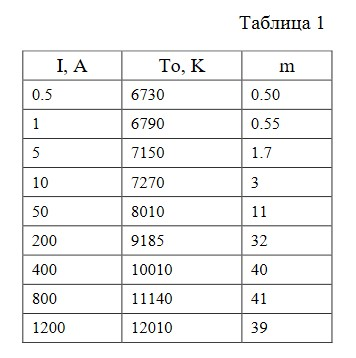
\includegraphics[scale=0.8]{source/Table1.jpg}
\end{figure}\par
\newpage
\begin{figure}[h]
	\centering
	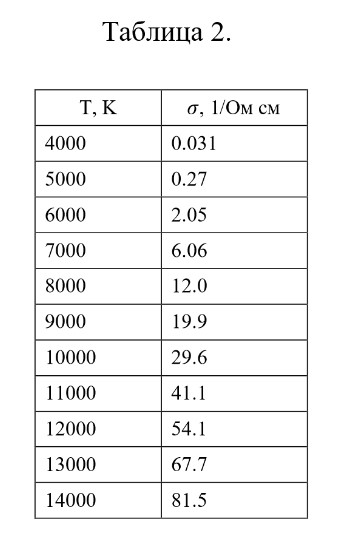
\includegraphics[scale=0.8]{source/Table2.jpg}
\end{figure}\par
\newpage
Параметры разряного контура:
\noindent$
R = 0.35\text{ см},\\
L_e = 12\text{ см},\\
L_k = 187 * 10^{-6}\text{ Гн},\\
C_k = 268 * 10^{-6}\text{ Ф},\\
R_k = 0.25\text{ Ом},\\
U_c = 1400\text{ В},\\
I_0 = 0..3\text{ А},\\
T_w = 2000\text{ К}
$\par

\section*{Теоритические сведения}
Метод Рунге-Кутты 4-го порядка точности.


\begin{equation*}
	y_{n+1} = y_n + \frac{k_1 + 2k_2 + 2k_3 + k_4}{6},
\end{equation*}

\begin{equation*}
	z_{n+1} = z_n + \frac{q_1 + 2q_2 + 2q_3 + q_4}{6}
\end{equation*}

\begin{equation*}
	k_1 = h_n f(y_n, z_n), ~~q_1 = h_n \varphi (y_n)
\end{equation*}

\begin{equation*}
	k_2 = h_n f (y_n + \frac{k_1}{2}, z_n + \frac{q_1}{2}),~~ q_2 = h_n \varphi(y_n + \frac{k_1}{2})
\end{equation*}

\begin{equation*}
	k_3 = h_n f (y_n + \frac{k_2}{2}, z_n + \frac{q_2}{2}), ~~q_3 = h_n \varphi(y_n + \frac{k_2}{2})
\end{equation*}

\begin{equation*}
	k_4 = h_n f (y_n + k_3, z_n + q_3, ~~q_4 = h_n \varphi(y_n + k_3)
\end{equation*}

\newpage
\section*{Реализация}
\begin{lstlisting}[caption=Интерполяция]
double Interpolation(double Y, List<double> tableY, List<double> table)
{
	int iMax = 0,
	iMin = 0;
	for (int i = 0; i < tableY.Count; i++)
	{
		if (Y > tableY[i])
			iMax = i;
		else
		{
			iMax = i;
			break;
		}
	}
	if (iMax == 0)
		iMax = 1;
	iMin = iMax - 1;
	return table[iMin] + (table[iMax] - table[iMin]) / (tableY[iMax] - tableY[iMin]) * (Y - tableY[iMin]);
}
\end{lstlisting}
\begin{lstlisting}[caption=Интегрирование]
double GetInt(double I, double arg)
{
	double tZero = Interpolation(I, arrI, arrTZero);
	TZeroForGraph = tZero;
	double m = Interpolation(I, arrI, arrM);
	double t = tZero + (tw - tZero) * (Math.Pow(arg, m));
	double sigma = Interpolation(t, arrT, arrSigma);
	return sigma * arg;
}

double CalculateIntegral(double I)
{
	double a = 0,
		b = 1,
		n = 100,
		h = (b - a) / n,
		result = (GetInt(I, a) + GetInt(I, b)) / 2,
		curr = 0;
	
	for (int k = 0; k < n - 1; k++)
	{
		curr += h;
		result += GetInt(I, curr);
	}
	return result * h;
}
\end{lstlisting}
\begin{lstlisting}[caption=Нахождение сопротивления]
double GetRp(double Le, double R, double I)
{
	double res = Le / (2 * Math.PI * Math.Pow(R, 2) * CalculateIntegral(I));
	return res;
}
\end{lstlisting}
\begin{lstlisting}[caption=Решение системы методом Рунге-Кутта]
double f(double I, double U, double Le, double R, double Lk, double Rk)
{
	RpForGraph = GetRp(Le, R, Math.Abs(I));
	return (U - (Rk + RpForGraph) * I) / Lk;
}

double g(double I, double Ck)
{
	return -I / Ck;
}

List<double> GetCoefs(double I, double U, double Le, double R, double Lk, double hn, double Rk, double Ck)
{
	double k1 = f(I, U, Le, R, Lk, Rk),
		q1 = g(I, Ck),
		k2 = f(I + hn * k1 / 2, U + hn * q1 / 2, Le, R, Lk, Rk),
		q2 = g(I + hn * k1 / 2, Ck),
		k3 = f(I + hn * k2 / 2, U + hn * q2 / 2, Le, R, Lk, Rk),
		q3 = g(I + hn * k2 / 2, Ck),
		k4 = f(I + hn * k3, U + hn * q3, Le, R, Lk, Rk),
		q4 = g(I + hn * k3, Ck);
	return new List<double>() { k1, k2, k3, k4, q1, q2, q3, q4 };
}

List<double> GetIAndU(double I, double U, double Le, double R, double Lk, double hn, double Rk, double Ck)
{
	List<double> coefs = GetCoefs(I, U, Le, R, Lk, hn, Rk, Ck);
	List<double> result = new List<double>() { 
		I + hn * (coefs[0] + 2 * coefs[1] + 2 * coefs[2] + coefs[3]) / 6,
		U + hn * (coefs[4] + 2 * coefs[5] + 2 * coefs[6] + coefs[7]) / 6
	};
	return result;
}
\end{lstlisting}

\section*{Результаты работы программы}
\begin{enumerate}
	\item Графики зависимости от времени импульса t: $I(t),U(t),R_p(t),$ произведения $I(t)R_p(t), T_0(t)$ при заданных выше параметрах. Указать шаг сетки.\\
	\begin{figure}[h]
		\centering
		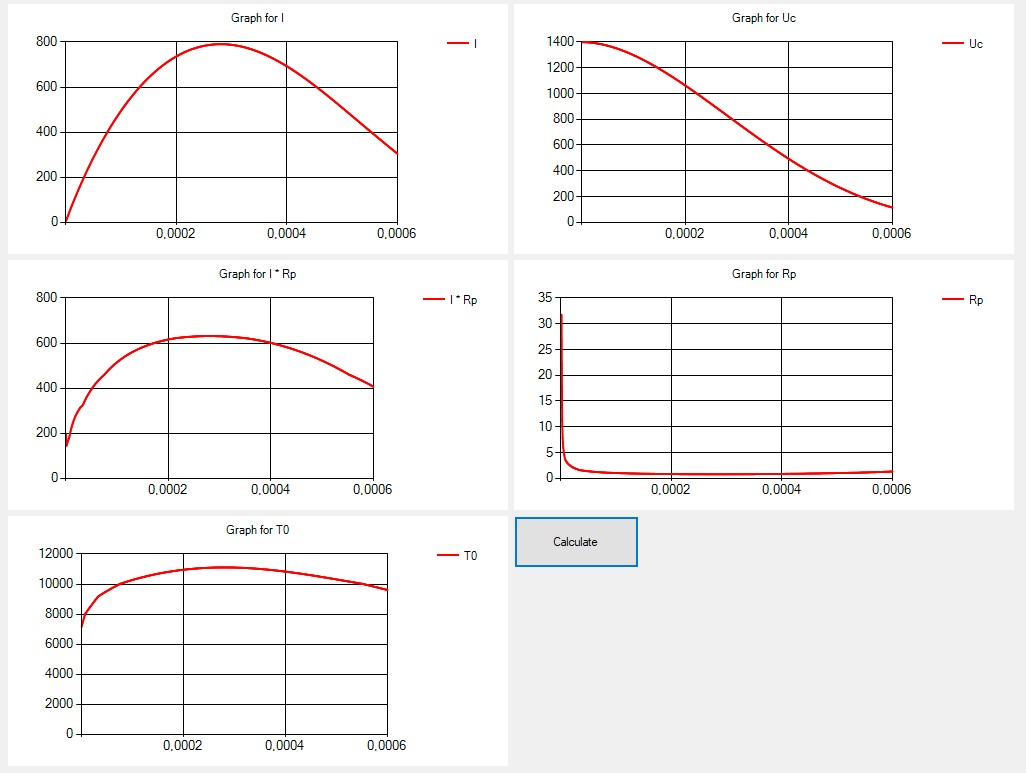
\includegraphics[scale=0.65]{source/test1.jpg}
	\end{figure}\par
	Шаг сетки - 1e-6
	\newpage
	\item График зависимости $I(t)$ при $R_k+R_p=0$. Обратить внимание на то, что в этом случае колебания тока будут незатухающими.\\
	\begin{figure}[h]
		\centering
		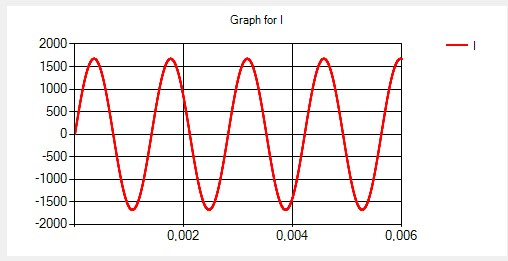
\includegraphics[scale=1]{source/test2.jpg}
	\end{figure}\par
	\item График зависимости $I(t)$ при $R_k + R_p = \text{const} = 200$ Ом в интервале значений 0 - 20 мкс.
	\begin{figure}[h]
		\centering
		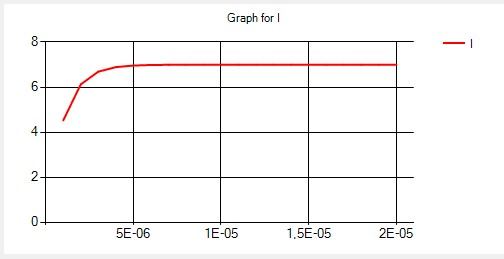
\includegraphics[scale=1]{source/test3.jpg}
	\end{figure}\par
	\item Результаты исследования влияния параметров контура $C_k, L_k, R_k$ на длительность импульса $t_{\text{имп}}$ апериодической формы. Длительность импульса определяется по кривой зависимости тока от времени на высоте $0.35I_{\text{max}}, I_{\text{max}}$ - значение тока в максимуме.\\
	График при начальных значениях:
	\begin{figure}[h]
		\centering
		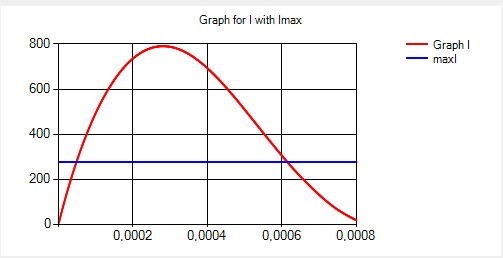
\includegraphics[scale=1]{source/test4.1.jpg}
	\end{figure}\par
	\newpage
	
	График при увеличении $C_k$ в 2 раза:
	\begin{figure}[h]
		\centering
		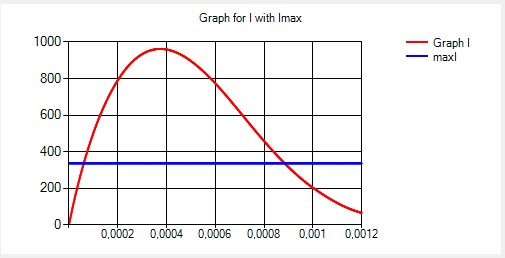
\includegraphics[scale=1]{source/test4.2.jpg}
	\end{figure}\par
	При увеличении $C_k$, $t_{\text{имп}}$ увеличивается.\\
	\newpage
	График при уменьшении $C_k$ в 2 раза:
	\begin{figure}[h]
		\centering
		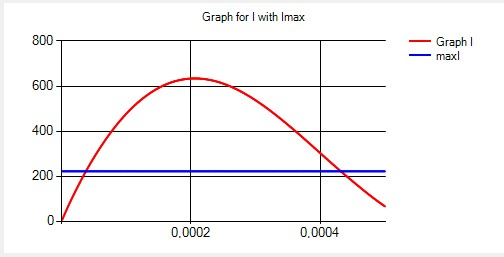
\includegraphics[scale=1]{source/test4.3.jpg}
	\end{figure}\par
	При уменьшении $C_k$, $t_{\text{имп}}$ уменьшается.\\
	
	График при увеличении $L_k$ в 2 раза:
	\begin{figure}[h]
		\centering
		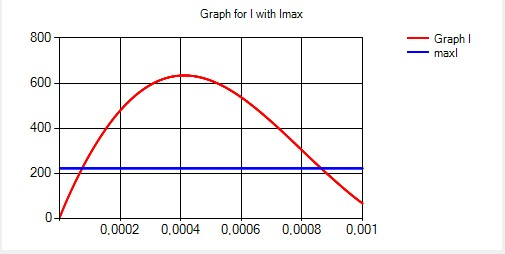
\includegraphics[scale=1]{source/test4.4.jpg}
	\end{figure}\par
	При увеличении $L_k$, $t_{\text{имп}}$ увеличивается.\\
	\newpage
	График при уменьшении $L_k$ в 2 раза:
	\begin{figure}[h]
		\centering
		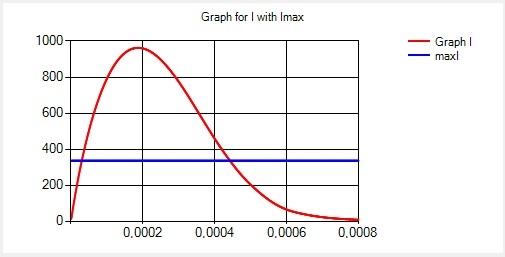
\includegraphics[scale=1]{source/test4.5.jpg}
	\end{figure}\par
	При уменьшении $L_k$, $t_{\text{имп}}$ уменьшается.\\
	
	График при увеличении $R_k$ в 5 раза:
	\begin{figure}[h]
		\centering
		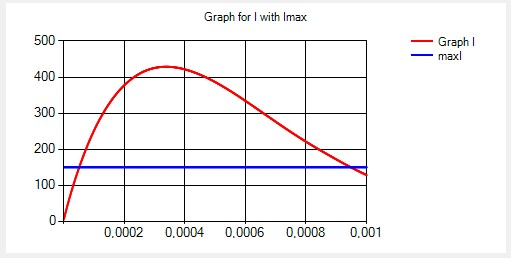
\includegraphics[scale=1]{source/test4.6.jpg}
	\end{figure}\par
	При увеличении $R_k$, $t_{\text{имп}}$ увеличивается.\\
	\newpage
	График при уменьшении $R_k$ в 5 раза:
	\begin{figure}[h]
		\centering
		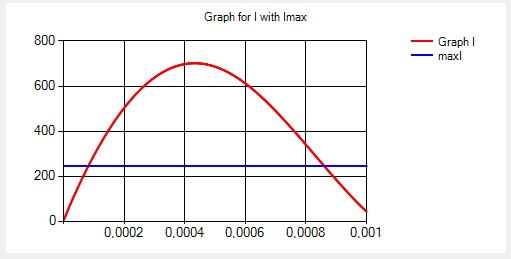
\includegraphics[scale=1]{source/test4.7.jpg}
	\end{figure}\par
	При уменьшении $R_k$, $t_{\text{имп}}$ уменьшается.\\
	
\end{enumerate}

\section*{Ответы на вопросы}
\begin{enumerate}
	\item Какие способы тестирования программы, кроме указанного в п.2, можете предложить ещё?\\
	Можно убрать лампу, тогда при большом значении параметра $R_k$ будет апериодическое затухание, а при небольшом - затухающие колебания.
	\item Получите систему разностных уравнений для решения сформулированной задачи неявным методом трапеций. Опишите алгоритм реализации полученных уравнений.\\
	$
	u_{n+1} = u_n + \int_{x_n}^{x_{n+1}}f(x, u(x)) dx\\
	u_{n+1} = u_n + \frac{h}{2}[f(x_n, y_n) + f(x_{n+1}, u_{n+1})] + O(h^2)\\ \\	
	\begin{cases}			
		\frac{dI}{dT} = \frac{U - (R_k + R_p(I))I}{L_k}\\
		\frac{dU}{dT} = \frac{- I}{C_k}
		
	\end{cases}\\ \\		
	I_{n+1} = I_n + \frac{h}{2}[\frac{U_n - (R_k + R_p(I_n))I_n}{L_k} + \frac{U_{n+1} - (R_k + R_p(I_{n+1}))I_{n+1}}{L_k}]\\
	U_{n+1} = U_n + \frac{h}{2} [-\frac{I_n}{C_k} - \frac{I_{n+1}}{C_k}] =
	U_n - \frac{h}{2}[\frac{I_n + I_{n+1}}{C_k}]\\
	\text{Подставляя $U_{n+1}$ в выражение для $I_{n+1}$}\\			
	I_{n+1} = I_n + \frac{h}{2L_k}[2U_n - (R_k + R_p(I_n) + \frac{h}{2C_k})I_n
	-(R_k + R_p(I_{n+1}) + \frac{h}{2C_k})I_{n+1}]\\
	\text{Получим уравнение вида}\\
	x = f(x)\\
	$
	Его можно решить методом простых итераций или методом Ньютона, после этого определить $U_{n+1}$.
	\item Из каких соображений проводится выбор численного метода того или иного порядка точности, учитывая, что чем выше порядок точности метода, тем он более сложен и требует, как правило, больших ресурсов вычислительной системы?\\
	Оценка для частного случая вида правой части дифференциального уравнения $\phi(x, u) \equiv \phi(x)$\\
	Если правая часть непрерывна и ограничена, и её четвёртые производные тоже, то использование метода Рунге-Кутта четвёртого порядка имеет смысл.\\
	Иначе, предельный порядок схемы Рунге-Кутта не может быть достигнут, и стоит использовать более простые схемы. 
\end{enumerate}



\end{document}









